% CausalVerify - NeurIPS 2026 Evaluations & Datasets Track
% Final anonymous submission build.

\documentclass{article}

% NeurIPS 2026 E&D Track. Keep anonymous for submission unless a separate
% single-blind decision is documented.
\PassOptionsToPackage{numbers, compress}{natbib}
\usepackage[eandd]{neurips_2026}
\usepackage[T1]{fontenc}
\usepackage[utf8]{inputenc}
\usepackage{microtype}

% Core packages
\usepackage{float}
\usepackage{booktabs}
\usepackage{multirow}
\usepackage{makecell}
\usepackage[dvipsnames]{xcolor}
\usepackage{colortbl}
\usepackage{tcolorbox}
\tcbuselibrary{skins, breakable}
\usepackage{enumitem}
\usepackage{tabularx}
\usepackage{array}
\usepackage{amsmath, amssymb}
\usepackage{pifont}
\usepackage{graphicx}
\graphicspath{{../figures/}{figures/}}
\usepackage{tikz}
\usetikzlibrary{positioning, arrows.meta, calc, fit, backgrounds, shapes.geometric}
\usepackage{caption}
\usepackage[hidelinks]{hyperref}
\usepackage{cleveref}

% Colors
\definecolor{passgreen}{HTML}{27AE60}
\definecolor{failred}{HTML}{E74C3C}
\definecolor{deepblue}{HTML}{2C3E50}
\definecolor{clrA}{HTML}{1565C0}   % dark blue - Prompt (A)
\definecolor{clrB}{HTML}{E65100}   % deep orange - Response (B)
\definecolor{clrC}{HTML}{2E7D32}   % forest green - Score (C)
\definecolor{lightblue}{HTML}{FFFFFF}
\definecolor{reasblue}{HTML}{D6EAF8}
\definecolor{instrpink}{HTML}{FDEDEC}
\definecolor{rowgray}{HTML}{F8F9FA}

% Heatmap cell colors (5-level blue-to-pink, matching paper palette)
\definecolor{heat90}{HTML}{D6EAF8}   % ≥90%  strong blue
\definecolor{heat75}{HTML}{EBF5FB}   % 75-89% light blue
\definecolor{heat60}{HTML}{F8F9FA}   % 60-74% neutral gray
\definecolor{heat40}{HTML}{FEF0F0}   % 40-59% light warm
\definecolor{heat0}{HTML}{FDEDEC}    % <40%   light pink

% Commands
\newcommand{\Lpass}{\textcolor{passgreen}{\ding{51}}}
\newcommand{\Lfail}{\textcolor{failred}{\ding{55}}}
\newcommand{\Lpart}{\textcolor{orange}{$\sim$}}
\newcommand{\model}[1]{\texttt{\small #1}}
\newcommand{\rid}{\textsc{rid}}
\newcommand{\bench}{\textsc{CausalVerify}}
\newcommand{\pp}{\,pp}

\newtcolorbox{finding}[2][]{
  enhanced, breakable,
  colback=white, colframe=deepblue,
  fonttitle=\bfseries\small,
  title={Finding #2},
  left=6pt, right=6pt, top=3pt, bottom=3pt, #1
}

\title{CausalVerify: An Execution-Grounded Benchmark for LLM\\ Causal Inference Workflows}
\author{Anonymous Author(s)}

% ─────────────────────────────────────────────────────────

\begin{document}

\maketitle

\begin{abstract}
Existing causal-inference benchmarks for LLMs often evaluate text
descriptions of methods or whether generated code can run. They rarely
test whether the executed workflow recovers the target causal estimate.
CausalVerify studies this verification problem by separating realistic
interpretation from verifiable computation. The benchmark draws on 259
published economics papers, each represented by a reconstructed research
question, data description, and institutional context, together with 100
fixed-seed synthetic scenarios that realise CSV datasets for
difference-in-differences (DID), event study (ES), instrumental variables
(IV), and regression discontinuity design (RDD). Experiment~A scores
method-family and direction agreement against four-LLM consensus labels.
Experiment~B runs model-written R code and checks whether the extracted
treatment-effect estimate matches a canonical estimator on the same
realised dataset. A calibration arm asks whether self-reported confidence
separates correct from incorrect workflows. On Experiment~B, seven
evaluated LLMs reach final L2b+ pass rates between 10\% and 88\%.
Execution ranking (L2b) agrees with coefficient recovery (L2b+) far
better than text-direction scoring (L4): Kendall $\tau=0.81$ and Spearman
$\rho=0.93$, versus Kendall $\tau$ between $-0.20$ and $0.10$ for L4. A
robustness run with Llama-3.3-70B-Instruct shows the same qualitative
gap, and reported confidence does not reliably separate correct from
incorrect workflows. Code, data, cached outputs, and a datasheet are
released with the submission.
\end{abstract}

\section{Introduction}

Evaluating LLMs for empirical causal inference is a verification
problem, not merely a text-scoring problem. A valid empirical claim
requires an estimand, an identification argument, an estimator,
executable analysis code, and a numerical result whose interpretation
matches the target causal quantity~\citep{rubin1974estimating,
rosenbaum1983central,holland1986statistics,pearl2009causality,
imbens2015causal,angrist2009mostly}. This structure exposes a failure mode that standard
LLM evaluations can miss: a model may name the right empirical design,
produce code that runs without error, and still estimate the wrong
coefficient. In applied research, such failures are more dangerous than
obvious failures because the response appears fluent, complete, and
confident while the causal claim remains unverified. This concern sits
within broader verification pressure in scientific publishing, where
more than 10{,}000 papers were retracted in 2023, a record high
reported by \citet{vannoorden2023retractions}. As LLMs move from text
assistance toward software engineering, scientific-analysis agents, and
laboratory-instrumentation control
~\citep{gao2023pal,yao2023react,schick2023toolformer,
liu2023agentbench,wu2023autogen,huang2024mlagentbench,
jimenez2024swe,majumder2024discoverybench,chen2024scienceagentbench,
xie2025autonomouslab},
causal-inference evaluation must ask not
only whether a model sounds right, but whether its executed workflow
recovers the right estimate.

Existing benchmarks capture only parts of this problem. Prior work
and benchmarks on LLM causal reasoning study causal direction, graph
reasoning, counterfactuals, correlation-to-causation judgments,
intervention design, surveys of benchmark validity, and real-world
identification tasks~\citep{kiciman2023causal,zecevic2023causalparrots,
jin2023cladder,jin2024corr2cause,chen2024clear,chi2024unveiling,
yang2024criticalreview,ma2025causalsurvey,zhou2024causalbench,
acharya2025causcibench,lee2025econcausal,shi2026intervenebench,
sawarni2026causalreasoningbenchmark}. Code benchmarks evaluate whether
programs can be synthesized, executed, or made to pass
tests~\citep{chen2021codex,austin2021program,hendrycks2021apps,
li2022alphacode,lu2021codexglue,cassano2023multiple,lai2023ds1000,
gu2024cruxeval,jimenez2024swe,jain2024livecodebench,
zhuo2024bigcodebench}. These
settings are valuable, but causal workflows require a stricter check:
after a model interprets a study, chooses a design, writes analysis
code, and reports a treatment effect, does the executed workflow
recover the intended estimate? This gap matters because code can
pass surface checks while remaining semantically
wrong~\citep{liu2023chatgptcode}.

We introduce \textsc{CausalVerify}, an execution-grounded benchmark for
LLM causal-inference workflows. The benchmark deliberately separates
ecological realism from executable verifiability. Real published papers
provide realistic institutional context, but rarely provide the cleaned
data, final runnable specification, and counterfactual treatment effect
needed for direct verification. We therefore use 259 published
economics papers to measure text-level agreement on method family and
effect direction, not as verified causal correctness. Conversely,
fixed-seed synthetic DGPs sacrifice some realism but provide executable
targets: 100 realised CSV datasets across difference-in-differences,
event study, instrumental variables, and regression discontinuity
designs~\citep{imbens1994identification,angrist1996identification,
thistlethwaite1960regression,imbens2008rdd,lee2010rdd,
calonico2014robust,mackinlay1997event,bertrand2004trust,
abadie2005semiparametric,callaway2021did,goodmanbacon2021did,
sun2021eventstudy,santanna2020drdid,roth2023trending}.
Models write R code, the
benchmark executes it, and L2b+ checks whether the extracted
treatment-effect estimate matches a canonical estimator on the same
realised dataset.

\textsc{CausalVerify} separates four signals that are often conflated:
textual interpretation, code executability, numerical coefficient
recovery, and self-assessed confidence. Across seven evaluated LLMs,
final L2b+ pass rates range from 10\% to 88\%. Execution success is
strongly aligned with coefficient recovery (Kendall $\tau = 0.81$,
Spearman $\rho = 0.93$), whereas text-direction agreement is weakly or
negatively aligned with Exp~B L2b+ ranking (Kendall $\tau \in [-0.20,
0.10]$). Execution is not sufficient---some code runs and estimates
the wrong coefficient---but it is a stronger proxy for execution-grounded
coefficient recovery under our reference-label construction than L4
direction agreement. A calibration arm further shows that naive
retrospective confidence reports do not cleanly separate correct from
incorrect workflows under our prompt,
connecting the benchmark to work on calibration, verbalized
uncertainty, selective prediction, and
self-checking~\citep{guo2017calibration,geifman2017selective,
jiang2021know,lin2022uncertaintywords,mielke2022linguistic,
kadavath2022know,kuhn2023semantic,manakul2023selfcheckgpt,
tian2023calibration,xiong2024uncertainty}. Our contributions are a
benchmark design separating real-paper agreement from executable
correctness, L2b+ as an execution-grounded coefficient-recovery
metric, and empirical evidence that plausible text, runnable code,
numerical correctness, and confidence can diverge sharply.

\begin{figure}[t]
  \centering
  % Source vector: ../figures/fig1_causalverify_overview.svg
  % PDF rendered from the SVG via rsvg-convert; PNG fallback also exists.
  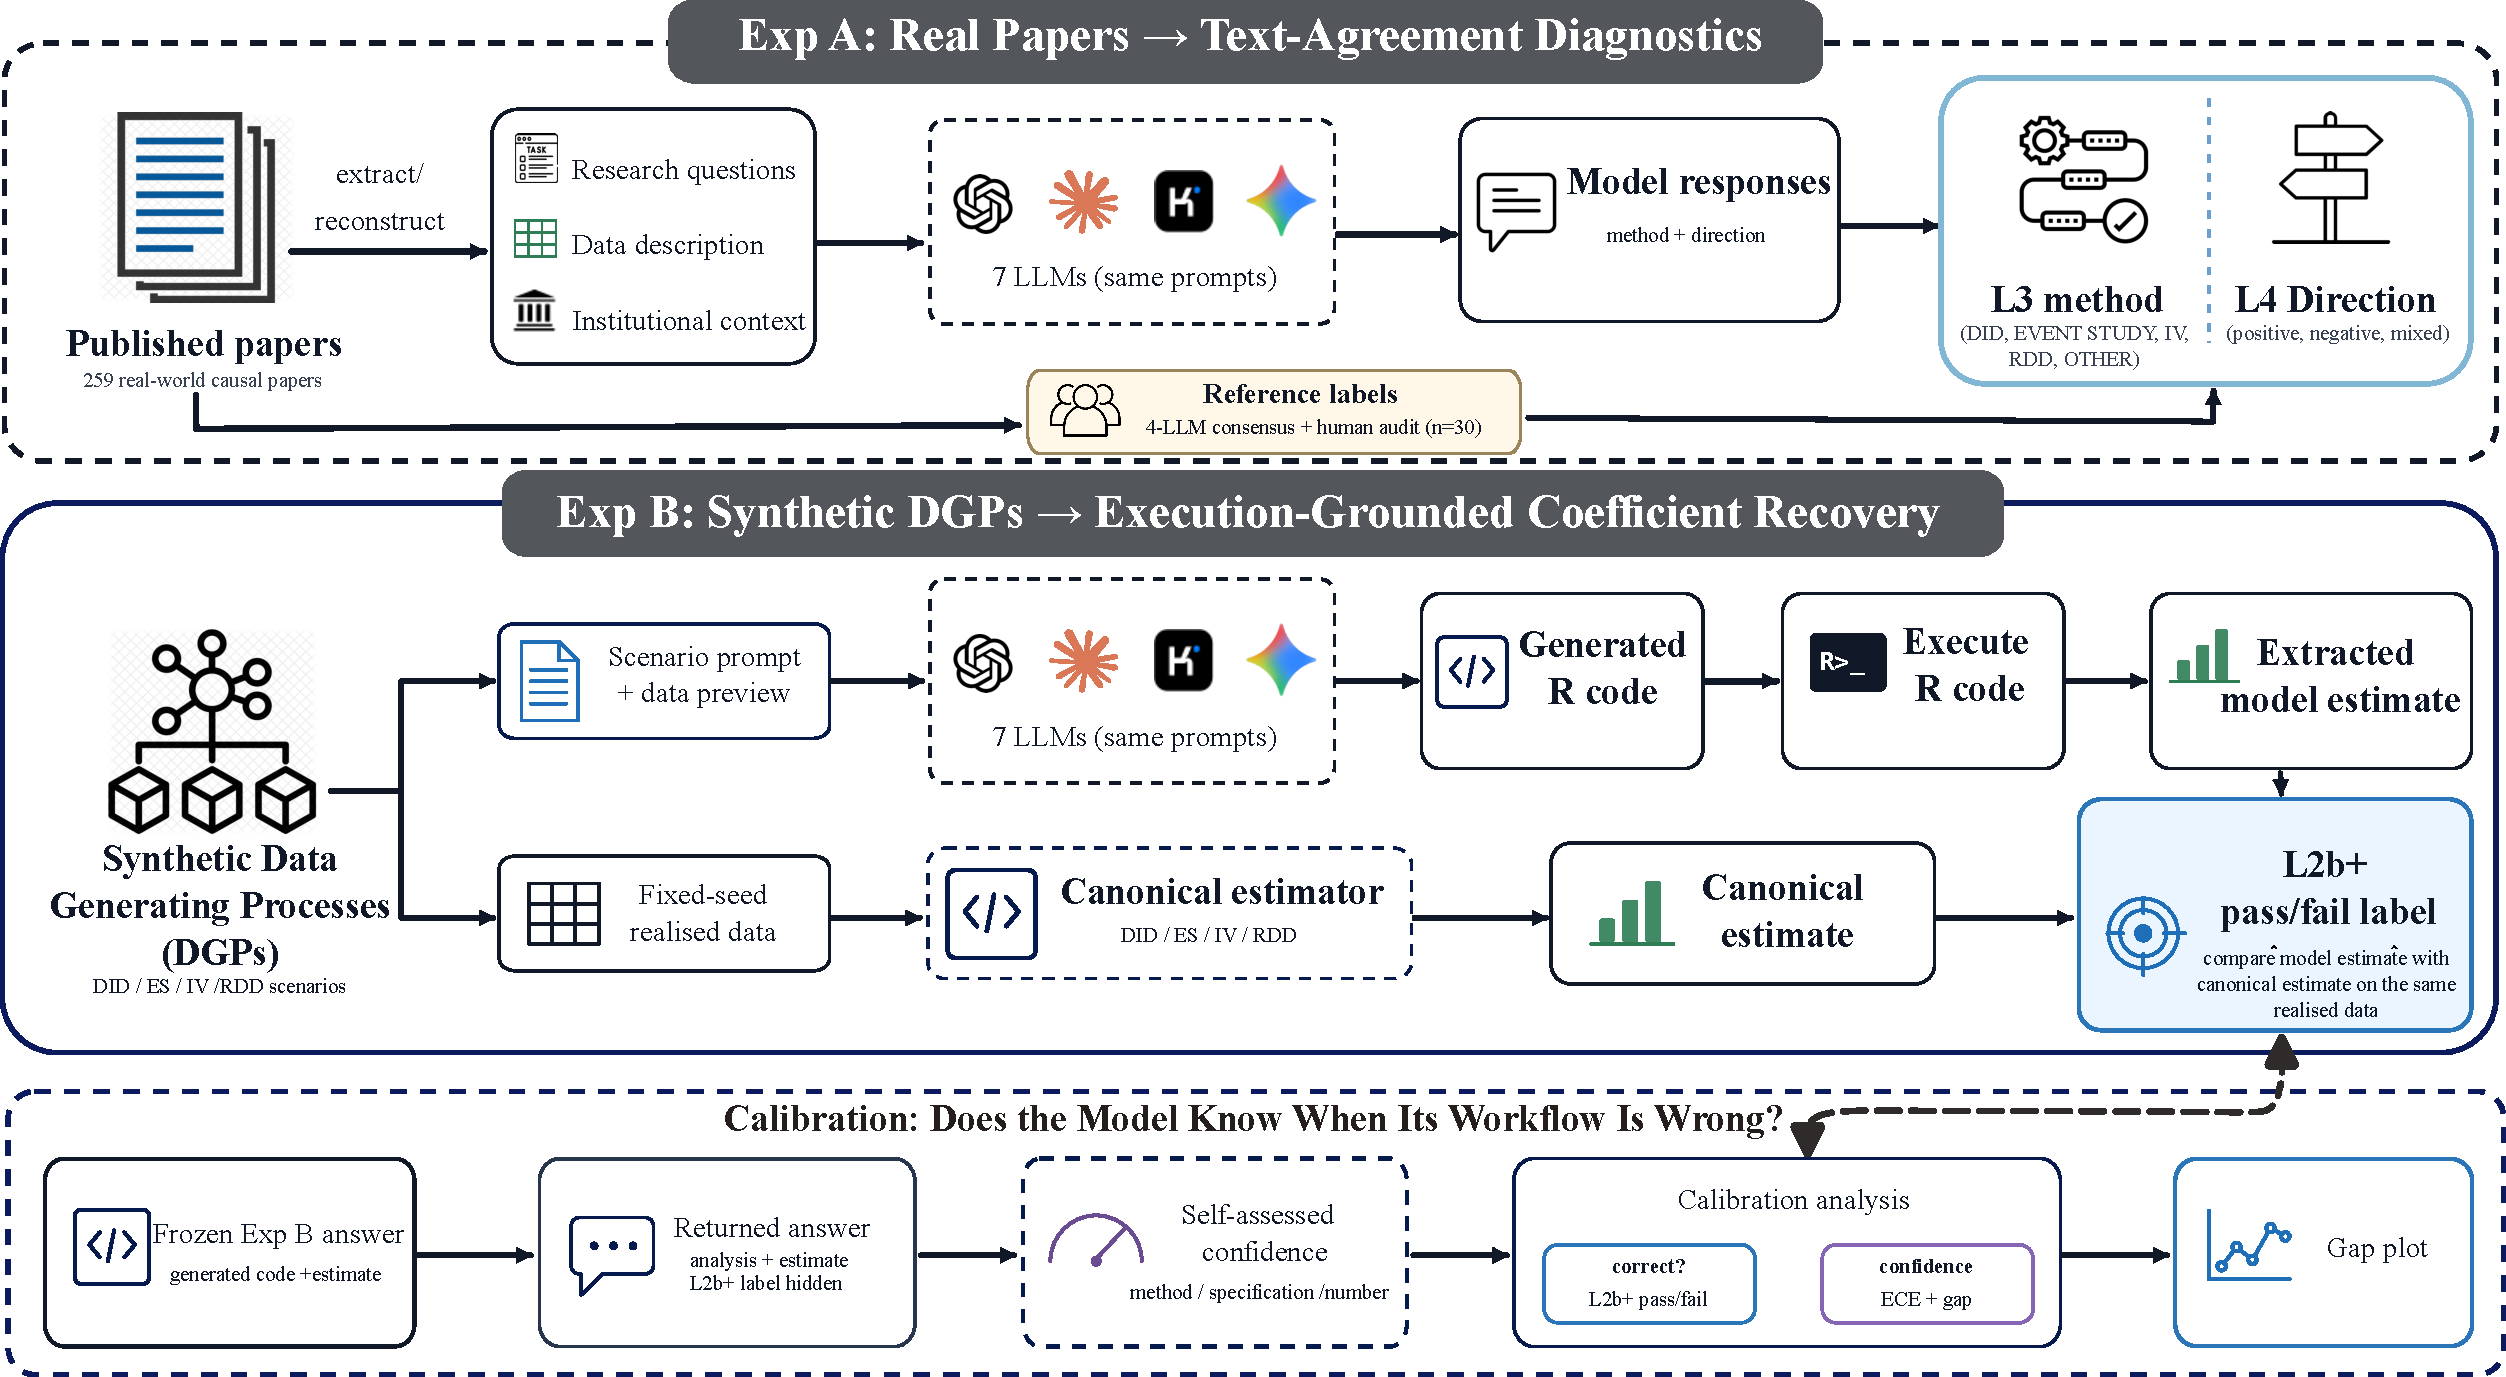
\includegraphics[width=\textwidth]{../figures/fig1_causalverify_overview.pdf}
  \caption{\bench{} benchmark overview. Exp~A uses published economics
  papers to form text-agreement tasks for method family and direction.
  Exp~B uses fixed-seed synthetic DGPs and realised datasets to evaluate
  executable model-written R workflows against canonical estimators.
  The calibration arm returns each model its own Exp~B answer and compares
  self-assessed confidence with L2b+ correctness.}
  \label{fig:benchmark_overview}
\end{figure}

\section{Related Work and Positioning}

Prior work evaluates important pieces of the LLM causal-analysis
workflow, but usually not the executed causal estimate. Causal
benchmarks test textual reasoning about direction, counterfactuals,
graphs, interventions, or identification. Code benchmarks test whether
generated programs execute or pass functional tests. Science-agent
benchmarks evaluate broader discovery or tool-use workflows.
\textsc{CausalVerify} differs in its verification target: the primary
correctness signal is not a text label or a generic program test, but
whether executed model-written analysis code recovers a
benchmark-defined target estimate on the realised dataset.

Among existing benchmarks, CauSciBench~\citep{acharya2025causcibench}
is nearest in scope: it evaluates end-to-end causal-analysis performance
over curated real, synthetic, and textbook tasks. \textsc{CausalVerify}
asks a complementary measurement question: when a model appears to
understand a causal task, which layer of the workflow is externally
verified? It separates real-paper text agreement, controlled-DGP
execution verification, and retrospective calibration rather than
collapsing them into a single causal-ability score.

Concurrent work by Sawarni et
al.~\citep{sawarni2026causalreasoningbenchmark} disentangles causal
identification from estimation on real-world datasets, and its finding
that strategy identification is easier than full specification is
consistent with our name-versus-compute gap. The methodological
difference is the unit of verification: \textsc{CausalVerify} verifies
generated and executed R code on controlled DGP data, extracts the
reported coefficient, and checks it against a realised-data canonical
estimate. This isolates the failure mode where code runs but computes
the wrong causal quantity. Recent workflow-oriented evaluations such as
BioMysteryBench
place models in bioinformatics environments with real data, tool
access, and objective final
answers~\citep{anthropic2026biomysterybench}; \bench{} is complementary:
it fixes a realised-data causal reference estimate so that
model-written causal code can be audited layer by layer rather than
graded only on a final answer. Table~\ref{tab:benchmark_comparison}
summarizes the distinction from adjacent benchmarks.

\begin{table}[H]
\centering
\caption{Comparison with adjacent benchmarks. The table reports
evaluation affordances rather than overall benchmark quality. A check
mark (\Lpass) indicates that a benchmark contains an explicit mechanism
for that dimension, not that it is superior in all respects.
\Lpart~= partial; \Lfail~= absent. $^{\dagger}$EconCausal counts
10{,}490 triplets across 2{,}595 studies (Lee et al.\ 2025).}
\label{tab:benchmark_comparison}
\footnotesize
\renewcommand{\arraystretch}{1.08}
\setlength{\tabcolsep}{2.5pt}
\begin{tabularx}{\textwidth}{lclcccc}
\toprule
\textbf{Benchmark} & \textbf{N} & \textbf{Target} &
\textbf{Real ctx.} & \textbf{Exec. coeff.} &
\textbf{Layered Dx} & \textbf{Self-assess.} \\
\midrule
CLadder / CORR2CAUSE~\citep{jin2023cladder,jin2024corr2cause} & 11k / 400 & Causal QA / direction
  & \Lpart & \Lfail & \Lfail & \Lfail \\
CausalBench~\citep{zhou2024causalbench} & 3 & Graph + effect
  & \Lfail & \Lfail & \Lpart & \Lfail \\
EconCausal~\citep{lee2025econcausal} & 10{,}490$^{\dagger}$ & Economic causal sign
  & \Lpass & \Lfail & \Lfail & \Lfail \\
CauSciBench~\citep{acharya2025causcibench} & 367 & End-to-end CI pipeline
  & \Lpass & \Lpart & \Lpart & \Lfail \\
InterveneBench~\citep{shi2026intervenebench} & 744 & Intervention design
  & \Lpass & \Lpart & \Lpart & \Lfail \\
CausalReasoningBench~\citep{sawarni2026causalreasoningbenchmark} & 173 & ID + estimate
  & \Lpass & \Lfail & \Lpart & \Lfail \\
Code benchmarks~\citep{chen2021codex,jimenez2024swe} & -- & Program tests
  & \Lfail & \Lpart & \Lpart & \Lfail \\
Discovery / science agents~\citep{majumder2024discoverybench,chen2024scienceagentbench} & 264 / 102 & Discovery workflow
  & \Lpass & \Lpart & \Lpart & \Lfail \\
\rowcolor{lightblue}
\bench{} & 259 + 100 & Causal workflow
  & \Lpass & \Lpass & \Lpass & \Lpass \\
\bottomrule
\end{tabularx}
\end{table}

\section{Benchmark Construction and Controls}

\textsc{CausalVerify} separates three evaluation regimes because no single
setting provides both ecological realism and executable truth. Real papers
test whether models parse applied research contexts, but their ground
truth is interpretive: the original cleaned data, exact runnable
specification, and counterfactual effect are usually unavailable. This
reflects the structure of empirical causal work, where claims depend on
the alignment of estimand, identification, estimator, and
data~\citep{angrist2009mostly,imbens2015causal}.
Synthetic DGPs give up some realism but make coefficient correctness
executable. Calibration then asks the deployment-facing question: when no
external verifier is available, can the model's own confidence serve as a
useful warning signal?

\paragraph{Exp A: real-paper context.}
Exp~A contains 259 retained published economics papers after excluding
two source failures. Each paper is represented by three reconstructed
fields: research question, data description, and institutional context.
Seven models are run on every paper, for 1813 outputs. Exp~A is
intentionally a text-level benchmark, comparable to prior LLM
causal-reasoning evaluations that score textual causal direction, method
recognition, sign judgments, or identification/estimation
judgments~\citep{jin2023cladder,jin2024corr2cause,lee2025econcausal,
sawarni2026causalreasoningbenchmark}. It measures method-family agreement
(L3) and direction agreement (L4) against four-LLM consensus reference
labels. The benchmark does not treat these labels as human-adjudicated
causal claims; instead, it uses real papers to test whether models read applied
study contexts in the same way as a structured consensus procedure.
The executable correctness endpoint is reserved for Exp~B.

\paragraph{Exp B: synthetic DGP execution.}
Exp~B contains 100 fixed-seed synthetic DGP scenarios across standard
applied causal-inference designs: difference-in-differences and event
studies, instrumental variables, and regression discontinuity
designs~\citep{callaway2021did,sun2021eventstudy,mackinlay1997event,
imbens1994identification,angrist1996identification,
thistlethwaite1960regression,imbens2008rdd,lee2010rdd}. The 100 scenarios
comprise 30 DID, 24 Event Study, 24 IV, and 22 RDD tasks; the realised
datasets and canonical estimates are fixed
before model evaluation. Models receive the research question, data
description, and a preview of the realised CSV, then produce runnable R
code. We execute the code and compare the extracted treatment-effect
estimate to a canonical estimator computed on the same realised dataset.
This realised-data comparison avoids penalizing models for finite-sample
deviations between the realised sample and the ideal DGP parameter.
Recent large-scale multi-analyst evidence shows that empirical claims can
vary under alternative defensible analyses of the same research question
and data~\citep{aczel2026analyticalrobustness}. We therefore treat the
Exp~B canonical estimator as a fixed reference path for executable
evaluation, not as the only scientifically defensible analysis.

\paragraph{Calibration: self-assessment.}
We attempt a calibration query for each frozen Exp~B output; response
availability yields 646 calibration records. The model is shown its own
previous analysis without the canonical estimate or pass/fail label and
asked to report confidence in the method choice, specification, and
numerical estimate. This is a
retrospective verbalized-confidence protocol rather than token-probability
calibration, connecting the benchmark to prior work on neural-network
calibration, LLM self-knowledge, and confidence
elicitation~\citep{guo2017calibration,kadavath2022know,
tian2023calibration,xiong2024uncertainty}. The resulting confidence is
compared to L2b+ correctness. This protocol deliberately mimics deployment:
a user may see a model's confidence even when no canonical estimator is
available.

\paragraph{Controls and claim boundaries.}
The benchmark uses a multi-stage evaluation pipeline rather than an
autonomous causal scientist. Separate stages construct contexts, audit
leakage, collect model responses, extract coefficients, aggregate labels,
and elicit calibration, reducing ``task writer = respondent = grader''
circularity. The synthetic scenarios are not free-form LLM inventions:
mathematical templates, treatment-effect signs, sample sizes, seeds,
realised CSV files, and canonical estimators are fixed by the benchmark.
Natural-language descriptions can vary, but a model cannot pass L2b+ by
guessing the sign or recognizing a phrase; it must produce code whose
estimated coefficient agrees with the realised-data reference. These
components support different claims: Exp~A is realistic but text-derived,
Exp~B is executable but synthetic, and calibration measures
confidence--correctness alignment. The benchmark is strongest when these
components are read together rather than collapsed into a single
leaderboard.

\begin{table}[t]
\centering
\caption{Benchmark controls. Each component supports a different claim
and protects against a different failure mode.}
\label{tab:controls}
\small
\renewcommand{\arraystretch}{1.12}
\setlength{\tabcolsep}{3pt}
\begin{tabularx}{\textwidth}{p{0.18\textwidth}p{0.40\textwidth}X}
\toprule
\textbf{Component} & \textbf{Implementation} & \textbf{Claim supported} \\
\midrule
Real context & 259 papers; reconstructed RQ/DD/IC; consensus reference
labels & Text-level method and direction agreement \\
Executable truth & 100 fixed-seed DGPs; realised CSVs; canonical
estimators & Numerical coefficient correctness \\
Role separation & Separate stages for construction, response, labeling,
extraction, calibration & Reduces circular grading \\
Leakage control & Method-name blacklist and prompt leakage audit &
Prevents trivial label recovery \\
Scorer audit & Coefficient extraction judge plus human validation audit
& Reduces brittle post-processing errors \\
Claim boundaries & Exp~A = agreement; Exp~B = execution; calibration =
confidence alignment & Prevents overclaiming \\
\bottomrule
\end{tabularx}
\end{table}

\section{Evaluation Layers}

The benchmark uses six scoring labels, but they apply to different
regimes. L1--L2b+ are Exp~B workflow-implementation layers, while L3/L4
are Exp~A text-agreement diagnostics. L1 checks that an output exists.
L2a checks for a parseable R code block. L2b executes the code with
\texttt{Rscript} in the fixed evaluation environment. L2b+ is the
execution-grounded correctness layer: it checks whether the extracted
treatment-effect estimate matches the realised-data canonical estimate
within the default relative-error tolerance. L3 measures method-family
agreement and L4 measures direction agreement against consensus reference
labels. Only L2b+ is a numerical correctness layer; L1/L2a are
bookkeeping diagnostics, L2b is execution, and L3/L4 are text agreement.

\paragraph{Why L2b+ uses a canonical estimator.}
The benchmark does not ask models to recover an ideal population
parameter directly. In finite samples, even a textbook estimator may
differ from the DGP parameter. We therefore compare model output to a
canonical estimator applied to the same realised dataset. For scalar
extracted estimate $\hat{\beta}_m$ and realised-data canonical estimate
$\hat{\beta}_c$, L2b+ passes when
\[
\frac{|\hat{\beta}_m-\hat{\beta}_c|}{|\hat{\beta}_c|} \le \tau ,
\]
with default tolerance $\tau=0.50$. Scenarios with
$|\hat{\beta}_c|<10^{-9}$ are marked unscoreable rather than divided. For
Event Study scenarios, accepted post-event windows and scale conversions
are frozen before scoring; valid cumulative post-event estimates are
accepted only when they can be deterministically converted to the
canonical per-day abnormal-return scale. This mapping is fixed before
model comparison.
Appendix~\ref{app:canonical_estimators} lists the canonical reference
estimate and accepted reported coefficient for each Exp~B method family.

\paragraph{Why L3/L4 are supporting metrics.}
Exp~A institutional context necessarily describes identifying variation,
so method family can often be inferred by a trained reader. We therefore
treat L3/L4 as agreement diagnostics, not verified causal correctness.
They are useful diagnostics of how models parse real research contexts, but the
load-bearing correctness evidence comes from Exp~B.

\paragraph{Scorer validation.}
A preliminary 30-case audit of L2b-pass/L2b+-fail examples found that
regex extraction produced many scorer-side failures. The final scorer
therefore uses a separate coefficient-extraction judge to identify the
reported treatment-effect estimate from executed stdout, followed by
deterministic numerical comparison against the canonical estimate. The
extraction judge sees the executed code, stdout, scenario context, and
method family, but not the evaluated model identity, canonical estimate,
or L2b+ label. A completed 50-cell blinded human audit of this extraction
instrument finds 90.9\% numeric agreement among human-scoreable
effect-present cells and 88.6\% agreement on the induced L2b+ pass/fail
decision; Appendix~\ref{app:l2b-judge-human} gives denominators and
disagreement cases. The judge can still err, so we treat L2b+ as an
audited execution-grounded metric rather than an infallible oracle.

\paragraph{Threshold choice.}
The default L2b+ tolerance is relative error at most 50\%. This
threshold is intentionally broad: it allows finite-sample and
implementation variation while still rejecting estimates that are off by
a factor large enough to change practical interpretation. The binary
threshold is a coarse workflow-success endpoint; the relative-error
profiles and tolerance sweep test whether conclusions depend on a single
cutoff.

\section{Results}

The results follow the same separation as the benchmark design. Exp~A first
shows what real-paper text agreement can and cannot tell us. Exp~B then
tests the executable claim: whether the model-written workflow recovers the
canonical estimate. Finally, calibration asks whether the models themselves
can identify when that workflow is wrong under a retrospective self-report
prompt.

\begin{figure}[t]
  \centering
  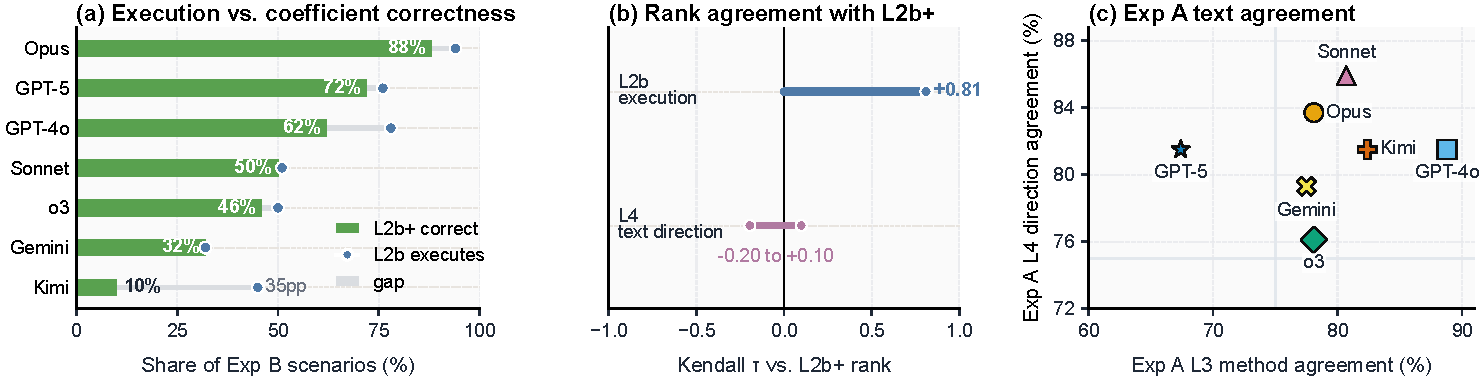
\includegraphics[width=\textwidth]{fig2_l2b_plus_cascade.pdf}
  \caption{Headline result. \textbf{(a)} L2b execution and L2b+ coefficient
  correctness are distinct. \textbf{(b)} L2b ranking tracks L2b+ correctness
  (Kendall $\tau=+0.81$), while L4 agreement against consensus direction
  labels has weak association with Exp~B L2b+ ranking
  ($\tau\in[-0.20,+0.10]$). \textbf{(c)} Exp~A L3/L4 agreement across the
  seven primary models; L3/L4 are diagnostics, not executable correctness
  endpoints.}
  \label{fig:headline}
\end{figure}

\paragraph{Finding 1: real-paper text agreement is useful but not decisive.}
On Exp~A, L3 is scoreable for 187/259 papers and L4 for 92/259 papers.
GPT-4o leads L3 (88.8\%), Claude Sonnet leads L4 (85.9\%), and GPT-5 is
lowest on L3 (67.4\%) but middle of the pack on L4 (81.5\%). The rankings
do not collapse to one textual ability score. Figure~\ref{fig:headline}(c)
summarizes the model-level separation between L3 method-family agreement and
L4 direction agreement, while Figure~\ref{fig:expa_text} breaks L3 down by
method family. Event Study has the lowest observed cross-model L3 mean in
this sample, but its smaller corpus size limits precision. The 30-paper
blinded human ambiguity audit reinforces this
interpretation: agreement with the 4-LLM consensus is 60.0\% for method
family and 47.6\% for direction. Exp~A is therefore best read as a
real-context text diagnostic, not as the paper's primary correctness
endpoint.

\begin{figure}[t]
\centering
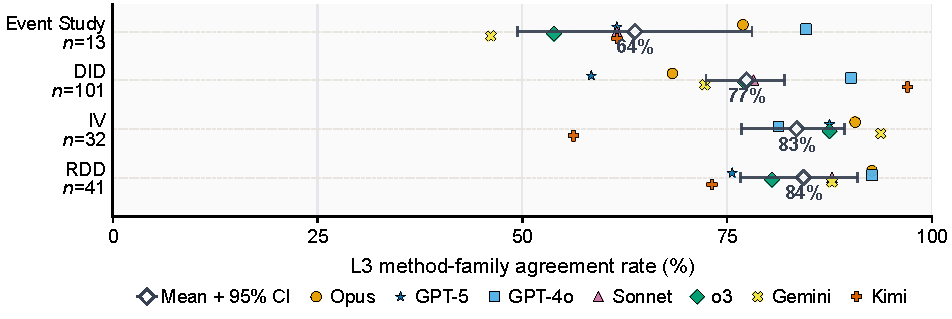
\includegraphics[width=0.90\textwidth]{fig3_method_dotplot.pdf}
\caption{Exp~A L3 method-family agreement by method family. Colored markers
show the seven model-level agreement rates; black diamonds and whiskers show
the cross-model mean with paper-cluster bootstrap 95\% intervals. Event Study
has the lowest observed mean (64\%, $n=13$) and the widest uncertainty. L3 is
a text-agreement diagnostic, not an executable correctness endpoint.}
\label{fig:expa_text}
\end{figure}

\paragraph{Finding 2: runnable code is not necessarily correct.}
Figure~\ref{fig:headline} shows that L2b execution and L2b+ correctness
separate the model panel. Final ES-aware canonical L2b+
rates span 10--88\% across the seven primary commercial models: Opus
88\%, GPT-5 72\%, GPT-4o 62\%, Sonnet 50\%, o3 46\%, Gemini 32\%, and
Kimi 10\%. This spread is invisible if evaluation stops at whether the
model wrote code.
Appendix~\ref{app:failure_taxonomy} decomposes Exp~B failures into execution,
reporting, target-coefficient, event-window, IV-stage, and RDD cutoff/sign
categories.

\begin{figure}[t]
\centering
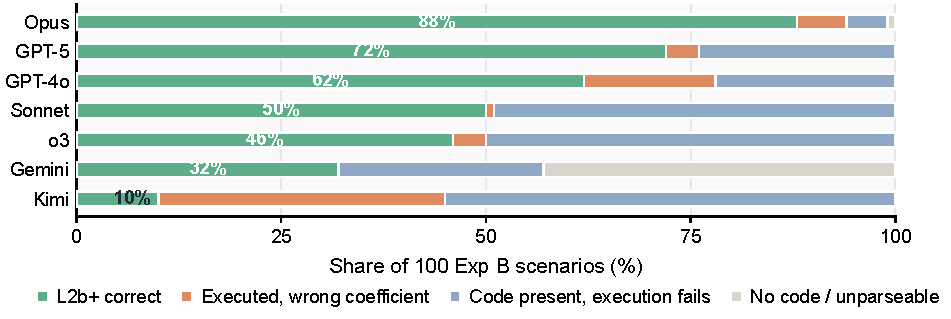
\includegraphics[width=0.90\textwidth]{fig4_cascade.pdf}
\caption{Execution cascade on Exp~B. Each bar partitions 100 scenarios for one
model
into L2b+ correct estimates, executed-but-wrong coefficients, execution
failures, and missing or unparseable code. The decomposition shows why
runnable code alone is not sufficient.}
\label{fig:cascade}
\end{figure}

\paragraph{Finding 3: execution ranking tracks numerical correctness.}
Across the seven models, the L2b ranking strongly matches the final L2b+
ranking (Kendall $\tau=+0.81$, Spearman $\rho=+0.93$).
Appendix~\ref{app:rank_stability} reports leave-one-model-out stability:
Kendall $\tau$ remains in $[0.733,0.867]$, with $\tau=0.714$ when adding
Llama as robustness-only. By contrast, L4 agreement against consensus
direction labels has weak or negative association with Exp~B L2b+
ranking ($\tau\in[-0.20,+0.10]$ across two frozen scorer variants).
Execution is not sufficient for correctness, but it is a much stronger
proxy for execution-grounded coefficient recovery under our reference-label
construction than text-level directional agreement. Because L2b+ is conditional
on execution, Appendix~\ref{app:expb-robustness} reports
$P(\mathrm{L2b+}\mid\mathrm{L2b})$ to separate execution failures from
executed-but-wrong estimates.

\paragraph{Finding 4: L2b+ rankings are not threshold artifacts.}
The L2b+ relative-error distributions show that stronger models
concentrate executed estimates near zero, while weaker models accumulate
large-error tails. Thus the ranking is better understood as a
distributional difference in numerical accuracy rather than an artifact
of the default 50\% cutoff. Appendix~\ref{app:additional-diagnostics}
reports the full relative-error profiles and tolerance sweep.
Appendix~\ref{app:tolerance_sweep} reports 10\%--100\% tolerance sweeps;
stricter cutoffs lower absolute pass rates but preserve the main
text-versus-execution separation.

\paragraph{Finding 5: naive retrospective confidence is a weak triage signal.}
Calibration asks each model to rate its own previous Exp~B output
without seeing the L2b+ pass/fail label. Actual L2b+ rates vary sharply, but
confidence gaps remain small for the main models. GPT-5 illustrates
the asymmetry: it is second on L2b+ but has a slightly negative
confidence gap. Under our retrospective confidence prompt, the
self-assessment signal therefore does not provide a reliable deployment
triage signal; this does not rule out stronger calibration interfaces.
Appendix~\ref{app:additional-diagnostics} reports reliability diagrams
for the retrospective confidence protocol.

\begin{table}[t]
\centering
\caption{Calibration summary against final L2b+ v2 correctness. Gap is
mean numerical confidence on correct outputs minus mean confidence on
incorrect outputs. Small gaps indicate weak triage value.}
\label{tab:calibration}
\small
\renewcommand{\arraystretch}{1.12}
\begin{tabular}{lccc}
\toprule
\textbf{Model} & \textbf{n} & \textbf{L2b+ v2} & \textbf{Conf. gap} \\
\midrule
Opus & 100 & 88.0 & +0.075 \\
GPT-5 & 99 & 71.7 & -0.045 \\
GPT-4o & 100 & 62.0 & +0.016 \\
Sonnet & 99 & 49.5 & -0.011 \\
o3 & 100 & 46.0 & -0.010 \\
Gemini & 48 & 31.2 & +0.234 \\
Kimi & 100 & 10.0 & +0.027 \\
\bottomrule
\end{tabular}
\end{table}

\begin{figure}[t]
\centering
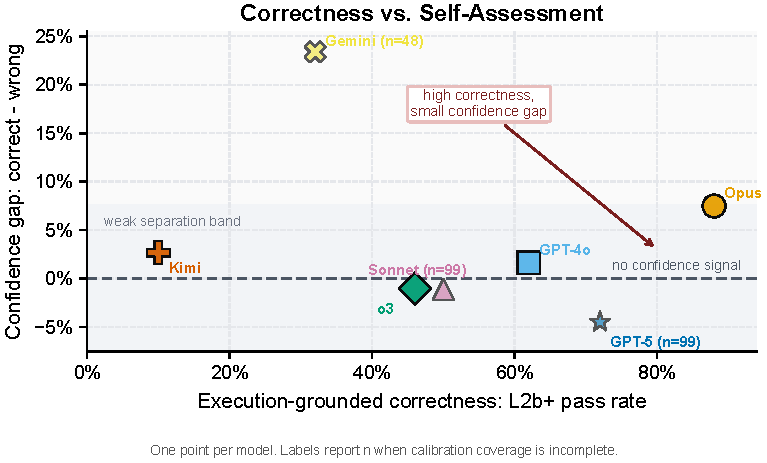
\includegraphics[width=0.82\textwidth]{calibration_gap_scatter.pdf}
\caption{Correctness versus self-assessment. Each point is one model.
The horizontal axis is execution-grounded L2b+ correctness; the vertical
axis is the mean numerical-confidence gap between correct and incorrect
workflows. High L2b+ accuracy does not imply a reliable confidence signal.}
\label{fig:calibration-gap}
\end{figure}

\paragraph{Robustness check: the execution--correctness gap reproduces for an open-weights model.}
As a single cross-vendor check, we evaluate Llama-3.3-70B-Instruct on the
same 100 Exp~B scenarios using the same prompt and scoring pipeline. It
reaches L2b $=41\%$ and final ES-aware L2b+ $=20\%$, placing it between
Kimi and Gemini and reproducing the same qualitative gap between runnable
code and numerically correct code. We treat this as a robustness check,
not a complete benchmark of the open-source ecosystem.

\section{Reproducibility and Human Audits}

The final submission build is tied to a frozen audit state. The released
artifacts include reconstructed Exp~A paper fields, four-LLM consensus
reference labels, 1813 Exp~A outputs, 700 primary Exp~B model-scenario
execution records, 100 realised CSV datasets with canonical-estimator
outputs, 646 calibration records, prompt hashes, scorer decision records,
and cached model responses. Deterministic scoring can be rerun without
new LLM calls; because commercial APIs are not bit-reproducible, the
release treats cached JSON outputs as the reproducible model-output layer.
Appendix~\ref{app:reproducibility} lists artifact paths and checksums.

Human annotation is intentionally an ambiguity audit rather than a
training or tuning input. A blinded 30-paper Exp~A slice was labeled from
the original PDFs after the automated benchmark freeze, without access to
Phase-2 LLM votes, consensus labels, or model outputs. These human labels
are not used to change the frozen consensus labels, prompts, model
outputs, or scoring thresholds. Agreement with the four-LLM consensus is
60.0\% for method family ($18/30$; Cohen's $\kappa=0.606$) and 47.6\% for
direction ($10/21$; Cohen's $\kappa=0.294$ among direction-scoreable
cases). This supports our interpretation of Exp~A as a real-context
agreement diagnostic with substantial ambiguity, while Exp~B supplies
executable correctness.

A separate blinded human audit validates the coefficient-extraction
instrument used for L2b+. The completed 50-cell audit finds 90.9\%
numeric agreement among human-scoreable effect-present cells and 88.6\%
agreement on the induced L2b+ pass/fail decision; Appendix~\ref{app:l2b-judge-human}
gives denominators and disagreement cases. This audit validates the
measurement instrument but does not change the frozen headline L2b+
rates.

\section{Limitations}

First, Exp~A labels are reference labels rather than L2b+ correctness
labels.
The final labels come from a four-LLM consensus after the final
paper-field reconstruction pass, and 100 disagreement cases remain
flagged for potential human adjudication. The completed blinded 30-paper
ambiguity audit agrees with the consensus on 60.0\% of method labels and
47.6\% of direction labels, indicating that real-paper method and
direction labels are noisy even under careful reading. This audit is
useful as an ambiguity check, but it does not make the 259-paper Exp~A
corpus fully human-adjudicated. We therefore use Exp~A to study text-level
agreement in real research contexts, not as verified causal correctness.
Because Exp~A uses published papers, we also cannot fully rule out
model familiarity with some studies from pretraining or public metadata.

Second, Exp~B is synthetic and structured. This is necessary for
executable reference estimates, but it measures whether models can
implement textbook workflows on known CSV data, not whether they can conduct an
entire empirical research project. The DGPs cover four major method
families but cannot represent all design choices in applied economics
and finance. In particular, Exp~B does not test literature review, data
cleaning, design selection from ambiguous field constraints, or
iterative robustness analysis.

Third, Exp~B fixes R as the execution backend. L2b+ therefore measures
executable workflow reliability under this released backend rather than
language-invariant causal ability; backend sensitivity across Python, Stata,
Julia, or other environments is an important extension.

Fourth, calibration is retrospective and prompt-specific. The protocol
tests whether models can assess their own prior outputs under our
confidence-elicitation prompt, not whether all possible uncertainty
interfaces would fail. Calibration coverage is also incomplete for some
models. The negative result should be read as evidence that naive
retrospective self-reported confidence is not enough, not as proof that no
calibrated interface can be designed.

Fifth, the evaluated model panel is limited. The primary panel consists
of closed or hosted frontier systems, which is appropriate for the
deployment question that motivates the paper but does not characterize
the full open-source ecosystem. We add one open-weights model as a
cross-vendor robustness check; a complete benchmark of multiple Llama,
Qwen, Mistral, DeepSeek, and domain-specific systems is left for future
work. Model-level rank correlations should also be read as descriptive
diagnostics over this evaluated panel, not population-level estimates
over all possible LLMs.

Sixth, L2b+ is an audited measurement instrument rather than an oracle.
It depends on the canonical specification, the relative-error tolerance,
event-study scale conversions, and coefficient extraction from executed
stdout. We mitigate these risks through frozen scorer rules, decision
records, and a completed coefficient-extraction human audit, but
individual-cell mistakes remain possible and should be treated as part
of the benchmark's measurement uncertainty.

Finally, the benchmark is intentionally single-shot and non-interactive.
Models receive fixed prompts and data previews, and the benchmark scores
the returned workflow rather than allowing extended human-in-the-loop
debugging or iterative robustness analysis. This design makes evaluation
reproducible and comparable across models, but it does not measure how a
supervised analyst might use an LLM over multiple rounds to improve a
causal study.

\section{Conclusion}

\textsc{CausalVerify} shows that the right unit of evaluation for
LLM-assisted causal inference is the workflow. A model may produce
plausible causal text and runnable code while still estimating the wrong
causal quantity. By separating real-paper agreement, execution,
coefficient recovery, and self-assessment, the benchmark exposes where
such workflows fail. Across seven evaluated LLMs, final L2b+ correctness
ranges from 10\% to 88\%, execution ranking tracks coefficient recovery
much better than L4 agreement against consensus direction labels, and naive
retrospective confidence reports do not reliably separate correct from
incorrect workflows under our prompt. For causal inference, the
question is therefore not whether an LLM can produce an analysis that
looks correct, but whether the workflow can be executed, checked against
a specified target, and accompanied by uncertainty signals that are
themselves audited.

\clearpage
\phantomsection
\label{sec:references-start}
\bibliographystyle{plainnat}
\bibliography{references}

\clearpage
\appendix

\section{Reproducibility Details}
\label{app:reproducibility}

\paragraph{Appendix roadmap.}
Appendix~A lists frozen artifacts and checksums. Appendix~B describes the
30-paper Exp~A ambiguity audit. Appendix~C reports Exp~B robustness
diagnostics: canonical-estimator targets, conditional
$P(\mathrm{L2b+}\mid\mathrm{L2b})$, rank-stability, tolerance sweep, scorer
evolution, and method-family breakdown. Appendix~D
contains the descriptive RID pilot. Appendix~E reports the 50-cell
coefficient-extraction human audit. Appendix~F contains additional
diagnostic figures moved from the main text.

The final submission build is tied to a complete audit state. The audit tag
\texttt{v11-freeze-2026-04-29} preserves the full provenance trail, while
\texttt{causalverify\_neurips2026.tex} provides a submission-length rendering
of the same claims. The final submission PDF checksum is documented in
\texttt{audit/SUBMISSION\_BUILD\_SUMMARY.md}.

\begin{table}[h]
\centering
\caption{Frozen artifacts used by the final submission build. The full audit
state remains available for inspection; the submission paper is a shorter
rendering of the same frozen claims.}
\label{tab:artifacts}
\small
\renewcommand{\arraystretch}{1.12}
\begin{tabular}{ll}
\toprule
\textbf{Claim} & \textbf{Frozen artifact} \\
\midrule
Exp A outputs & \texttt{experiments/exp\_a/outputs/} \\
Exp A scores & \texttt{experiments/exp\_a/auto\_scores.csv} \\
Exp B L2b+ & \texttt{l2b\_plus\_scores\_canonical\_judge\_v2.csv} (primary 7; Llama R6 retained) \\
Calibration & \texttt{calibration\_scores.csv}, \texttt{calibration\_summary\_v2.json} \\
Human validation & \texttt{audit/human\_gold/human\_vs\_llm\_consensus.md} \\
Paper checksum & \texttt{audit/SUBMISSION\_BUILD\_SUMMARY.md} \\
Gate evidence & \texttt{audit/V11\_ACCEPTANCE\_GATES.md} \\
\bottomrule
\end{tabular}
\end{table}

\section{Human Annotation Details}
\label{app:human}

The repository contains a paper-native labeling protocol and a completed
blinded 30-paper ambiguity audit slice. The annotator labeled method family and
direction from the original PDFs without access to Phase-2 LLM votes, consensus
labels, or model outputs. One target paper (\texttt{paper\_159}) was excluded
because the available PDF was appendix-only; \texttt{paper\_17} was added as a
blinded replacement from the unsealed sample manifest, which contains only
paper ID, difficulty tier, and PDF path. These human labels are not used to
silently change the frozen Exp~A labels. Human adjudication was conducted after
the automated benchmark freeze as an ambiguity audit, not as a training,
prompting, or tuning input; the labels are not used to construct prompts,
select model outputs, or tune scoring thresholds.

\section{Exp B Robustness Details}
\label{app:expb-robustness}

This appendix reports supporting diagnostics for Exp~B. These tables are
derived from \texttt{l2b\_plus\_scores\_canonical\_judge\_v2.csv} and do not
replace the frozen headline L2b+ rates in the main text.

\subsection{Canonical estimators for Exp B}
\label{app:canonical_estimators}

L2b+ compares the model-reported estimate to a fixed realised-data reference
estimate. The canonical estimator is a benchmark-defined reference path for
executable evaluation, not a claim that only one empirical analysis is
scientifically defensible. It is also distinct from the structural DGP
parameter used to simulate the data.

\begin{table}[h]
\centering
\caption{Benchmark-defined canonical estimators for Exp~B L2b+ scoring.}
\label{tab:canonical-targets}
\scriptsize
\renewcommand{\arraystretch}{1.10}
\setlength{\tabcolsep}{3pt}
\begin{tabularx}{\textwidth}{lXXXX}
\toprule
\textbf{Method} & \textbf{Canonical reference estimate} &
\textbf{Accepted model-reported coefficient} &
\textbf{Common non-target coefficients} & \textbf{Scope limitation} \\
\midrule
DID & TWFE coefficient on \texttt{treat\_x\_post} after unit and period
demeaning & \texttt{treat\_x\_post}, \texttt{treated:post}, or equivalent
treatment-by-post effect & \texttt{treated} main effect, \texttt{post} main
effect, placebo or pretrend coefficient & Clean benchmark DID template, not a
full benchmark of staggered or heterogeneous-treatment DID estimators \\
Event Study & Market-model coefficient on \texttt{event\_day >= 0}; ES-aware
v2 accepts frozen integer post-window conversions to this per-day scale &
Explicit post-event AAR/CAR that can be deterministically converted to the
canonical scale & Pre-event coefficient, arbitrary non-frozen window,
diagnostic or placebo return & Fixed benchmark window mapping, not a universal
event-study estimand \\
IV & Realised-data 2SLS coefficient on \texttt{x}, instrumented by
\texttt{z}, with controls exogenous when present & Second-stage coefficient on
\texttt{x} or the named endogenous variable & First-stage coefficient on
\texttt{z}, reduced form, or control coefficient & Tests implementation of the
IV estimand; does not validate exclusion restriction or weak-instrument
diagnostics \\
RDD & Local-linear cutoff effect on the realised data: coefficient on
\texttt{treated} near cutoff 0.5 with running-variable slope and interaction &
Treatment, above-cutoff, or discontinuity coefficient consistent with benchmark
direction & Density test, bandwidth statistic, unrelated global polynomial
trend, placebo cutoff estimate & Fixed benchmark RDD reference, not an
exhaustive comparison of bandwidth or inference choices \\
\bottomrule
\end{tabularx}
\end{table}

Because L2b+ requires code execution, raw L2b--L2b+ association is partly
structural. Table~\ref{tab:conditional-l2b} therefore reports the conditional
metric $P(\mathrm{L2b+}\mid \mathrm{L2b})$, which asks whether executed code
computes the right coefficient.

\begin{table}[h]
\centering
\caption{Conditional Exp~B correctness among executed outputs. ``Wrong after
execution'' is L2b count minus L2b+ v2 count.}
\label{tab:conditional-l2b}
\small
\renewcommand{\arraystretch}{1.08}
\begin{tabular}{lrrrrr}
\toprule
\textbf{Model} & \textbf{L2b} & \textbf{L2b+} &
\textbf{Wrong after exec.} & \textbf{$P$(L2b+|L2b)} & \textbf{Gap} \\
\midrule
Opus & 94 & 88 & 6 & 93.6\% & 6 pp \\
GPT-5 & 76 & 72 & 4 & 94.7\% & 4 pp \\
GPT-4o & 78 & 62 & 16 & 79.5\% & 16 pp \\
Sonnet & 51 & 50 & 1 & 98.0\% & 1 pp \\
o3 & 50 & 46 & 4 & 92.0\% & 4 pp \\
Gemini & 32 & 32 & 0 & 100.0\% & 0 pp \\
Kimi & 45 & 10 & 35 & 22.2\% & 35 pp \\
\bottomrule
\end{tabular}
\end{table}

\subsection{Exp B failure-taxonomy diagnostic}
\label{app:failure_taxonomy}

We also audit the non-L2b+ mass with a conservative rule-based taxonomy. The
taxonomy is diagnostic rather than a scoring replacement: it distinguishes
missing or unparseable code, execution failures, executed-but-unreported
effects, wrong target coefficients, event-window or scale mismatches, IV stage
errors, and RDD cutoff or sign-convention issues. Ambiguous cases are left
uncategorized rather than forced into a narrow label.

\begin{table}[h]
\centering
\caption{Exp~B failure-taxonomy diagnostic for the primary seven models.
Counts are over the 340 non-L2b+ cells and use existing frozen outputs,
scores, and judge-cache metadata.}
\label{tab:failure-taxonomy}
\small
\renewcommand{\arraystretch}{1.08}
\begin{tabular}{lrr}
\toprule
\textbf{Failure category} & \textbf{Count} & \textbf{Share of failures} \\
\midrule
Execution failure & 230 & 67.6\% \\
No code or unparseable code & 44 & 12.9\% \\
Executed wrong coefficient & 26 & 7.6\% \\
Coefficient not reported & 15 & 4.4\% \\
Event-window or scale mismatch & 11 & 3.2\% \\
IV first-stage or wrong-stage output & 5 & 1.5\% \\
RDD cutoff/sign convention & 3 & 0.9\% \\
Other target-specific categories & 6 & 1.8\% \\
\bottomrule
\end{tabular}
\end{table}

\subsection{Rank-stability diagnostic}
\label{app:rank_stability}

The rank correlations in Figure~\ref{fig:headline} are descriptive
model-level diagnostics over seven primary models rather than population-level
estimates. To assess panel sensitivity, we recompute Kendall $\tau$ and
Spearman $\rho$ after leaving out each model in turn. The leave-one-model-out
Kendall range is $0.733$--$0.867$ and the Spearman range is
$0.886$--$0.943$. Adding Llama-3.3-70B-Instruct as a robustness-only eighth
model gives Kendall $\tau=0.714$ and Spearman $\rho=0.881$, while the primary
leaderboard remains the seven-model panel.

\begin{table}[h]
\centering
\caption{Rank-stability diagnostic for the Exp~B model-level correlations.
Primary-panel rows summarize the audit table in
\texttt{paper/tables/exp\_b\_rank\_stability\_primary7.csv}; the Llama row is
robustness-only and does not enter the primary leaderboard.}
\label{tab:rank-stability}
\small
\renewcommand{\arraystretch}{1.08}
\begin{tabular}{lccc}
\toprule
\textbf{Diagnostic} & \textbf{$N$ models} & \textbf{Kendall $\tau$} &
\textbf{Spearman $\rho$} \\
\midrule
Primary seven-model baseline & 7 & 0.810 & 0.929 \\
Leave-one-model-out range & 6 each & 0.733--0.867 & 0.886--0.943 \\
Primary seven plus Llama robustness-only & 8 & 0.714 & 0.881 \\
\bottomrule
\end{tabular}
\end{table}

\begin{table}[h]
\centering
\caption{Scorer evolution on Exp~B. Regex extraction is retained as a legacy
diagnostic; the final headline uses the ES-aware v2 score. Entries are pass
rates in percentage points.}
\label{tab:scorer-evolution}
\small
\renewcommand{\arraystretch}{1.08}
\begin{tabular}{lrrrr}
\toprule
\textbf{Model} & \textbf{Regex} & \textbf{Judge} &
\textbf{ES-aware v2} & \textbf{v2--Judge} \\
\midrule
Opus & 64 & 71 & 88 & +17 \\
GPT-5 & 29 & 59 & 72 & +13 \\
GPT-4o & 28 & 50 & 62 & +12 \\
Sonnet & 27 & 31 & 50 & +19 \\
o3 & 18 & 37 & 46 & +9 \\
Gemini & 15 & 29 & 32 & +3 \\
Kimi & 6 & 8 & 10 & +2 \\
\bottomrule
\end{tabular}
\end{table}

\begin{table}[h]
\centering
\caption{L2b+ v2 by model and method family. Each cell reports
passes/available scenarios.}
\label{tab:l2b-method}
\small
\renewcommand{\arraystretch}{1.08}
\begin{tabular}{lrrrr}
\toprule
\textbf{Model} & \textbf{DID} & \textbf{ES} & \textbf{IV} & \textbf{RDD} \\
\midrule
Opus & 29/30=97\% & 19/24=79\% & 23/24=96\% & 17/22=77\% \\
GPT-5 & 20/30=67\% & 17/24=71\% & 23/24=96\% & 12/22=55\% \\
GPT-4o & 25/30=83\% & 13/24=54\% & 15/24=62\% & 9/22=41\% \\
Sonnet & 20/30=67\% & 21/24=88\% & 3/24=12\% & 6/22=27\% \\
o3 & 8/30=27\% & 12/24=50\% & 16/24=67\% & 10/22=45\% \\
Gemini & 14/30=47\% & 5/24=21\% & 13/24=54\% & 0/22=0\% \\
Kimi & 5/30=17\% & 4/24=17\% & 1/24=4\% & 0/22=0\% \\
\bottomrule
\end{tabular}
\end{table}

\subsection{Tolerance-sweep diagnostic}
\label{app:tolerance_sweep}

The binary L2b+ endpoint uses a broad default relative-error tolerance of
50\%. To check whether the qualitative conclusion depends on this cutoff, we
recompute primary-seven pass rates at 10\%, 25\%, 50\%, 75\%, and 100\%. The
sweep is used as a robustness diagnostic; the frozen headline results continue
to use the default 50\% tolerance. Table~\ref{tab:tolerance-sweep} reports
all-scenario pass rates, so non-executing outputs remain failures.

\begin{table}[h]
\centering
\caption{Tolerance-sweep diagnostic for Exp~B L2b+ scoring. Each cell reports
the pass rate out of 100 scenarios; parentheses give the model rank at that
tolerance. The 50\% column is the frozen headline threshold.}
\label{tab:tolerance-sweep}
\small
\renewcommand{\arraystretch}{1.08}
\begin{tabular}{lccccc}
\toprule
\textbf{Model} & \textbf{10\%} & \textbf{25\%} & \textbf{50\%} &
\textbf{75\%} & \textbf{100\%} \\
\midrule
Opus & 72\% (1) & 84\% (1) & 88\% (1) & 88\% (1) & 88\% (1) \\
GPT-5 & 64\% (2) & 71\% (2) & 72\% (2) & 72\% (2) & 72\% (2) \\
GPT-4o & 53\% (3) & 59\% (3) & 62\% (3) & 63\% (3) & 63\% (3) \\
Sonnet & 42\% (4) & 48\% (4) & 50\% (4) & 50\% (4) & 50\% (4) \\
o3 & 38\% (5) & 44\% (5) & 46\% (5) & 47\% (5) & 47\% (5) \\
Gemini & 32\% (6) & 32\% (6) & 32\% (6) & 32\% (6) & 32\% (6) \\
Kimi & 9\% (7) & 9\% (7) & 10\% (7) & 13\% (7) & 14\% (7) \\
\bottomrule
\end{tabular}
\end{table}

\clearpage
\section{RID Pilot Ablation}
\label{app:rid-pilot}

Experiment~C is a small descriptive pilot that reruns a 10-paper subset under
the \rid{} pre-commitment protocol. It is not used for the headline benchmark
claims, because $N=10$ per model is too small for model-level inference. We
include it only as an audit artifact showing how pre-commitment can change
text-level L3/L4 outcomes in either direction.

\begin{figure}[H]
\centering
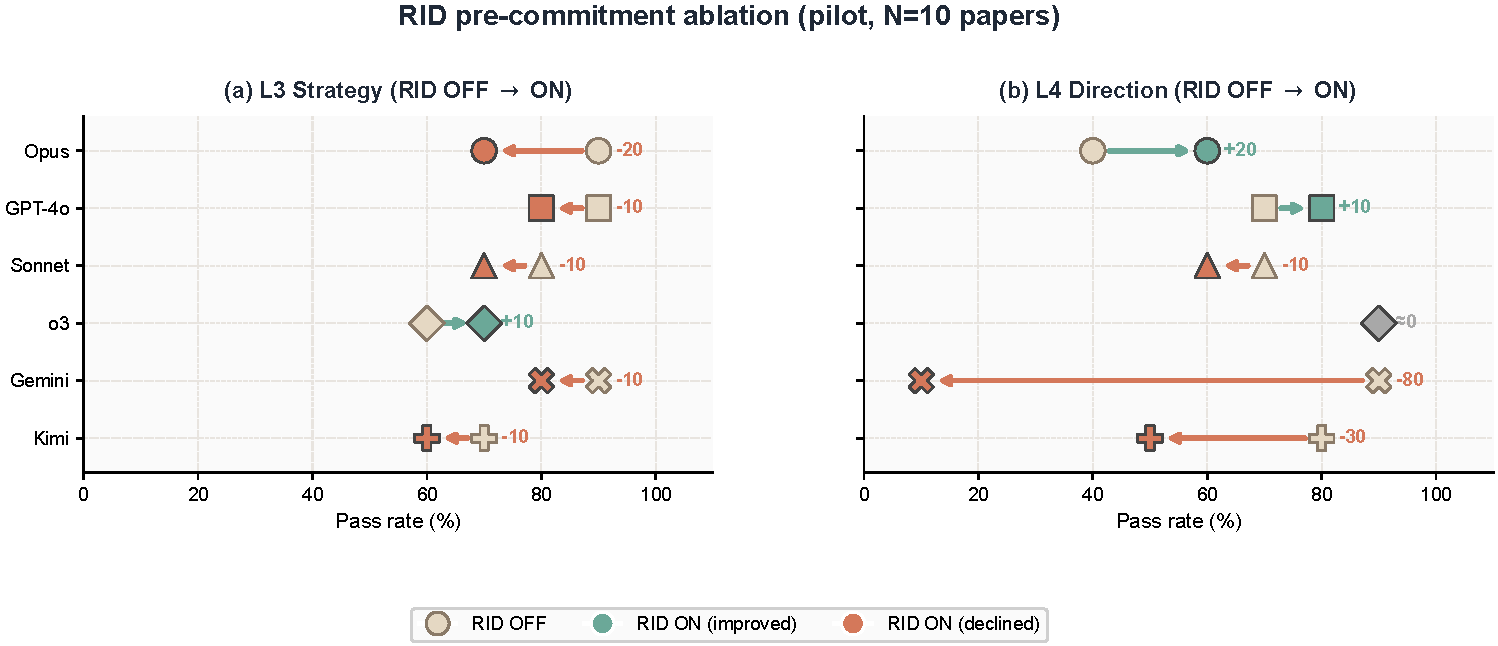
\includegraphics[width=0.98\textwidth]{fig_rid_pilot.pdf}
\caption{RID pre-commitment ablation pilot ($N=10$ papers per model,
descriptive only). Dots compare RID OFF and RID ON pass rates for L3 strategy
and L4 direction. No individual comparison is statistically significant; the
pilot is retained as an audit artifact rather than as evidence for the main
claims.}
\label{fig:rid-pilot}
\end{figure}

\section{Coefficient-Extraction Human Audit}
\label{app:l2b-judge-human}

The coefficient-extraction judge is a measurement instrument: it identifies
the scalar treatment-effect coefficient from executed R code/stdout before
L2b+ compares that coefficient to the canonical estimator. The repository
contains a blinded human-validation audit in
\texttt{audit/l2b\_judge\_human\_validation/}. The annotation form hides model
identity, L2b+ label, canonical estimate, judge effect, regex effect, and
ranking information. The completed audit covers 50 primary-panel L2b=1 cells
sampled with seed 20260502: DID 13, Event Study 12, IV 11, and RDD 14. Among
comparable audited cells, it found 90.9\% numeric agreement and 88.6\%
agreement on the induced L2b+ pass/fail decision. Disagreements concentrate in
event-study window choices and RDD sign/printing ambiguities. This audit
validates the coefficient-extraction instrument; it does not change the frozen
headline L2b+ rates.

\paragraph{Disagreement categories.}
Most disagreements arise from two sources: (i) Event Study outputs that
report a cumulative post-event window rather than the canonical per-day
scale, and (ii) RDD outputs where printed signs, jump orientation, or
robustness estimates make the main effect ambiguous. These cases motivate
treating L2b+ as an audited measurement instrument rather than an
infallible oracle.

\section{Additional Diagnostics}
\label{app:additional-diagnostics}

This appendix collects supporting diagnostic figures for the main results.
The main text reports the headline conclusions; the relative-error profiles,
calibration reliability diagrams, and L4 scorer-operationalization diagnostic
below support those conclusions but are not required for the central
correctness argument.

\begin{figure}[h]
\centering
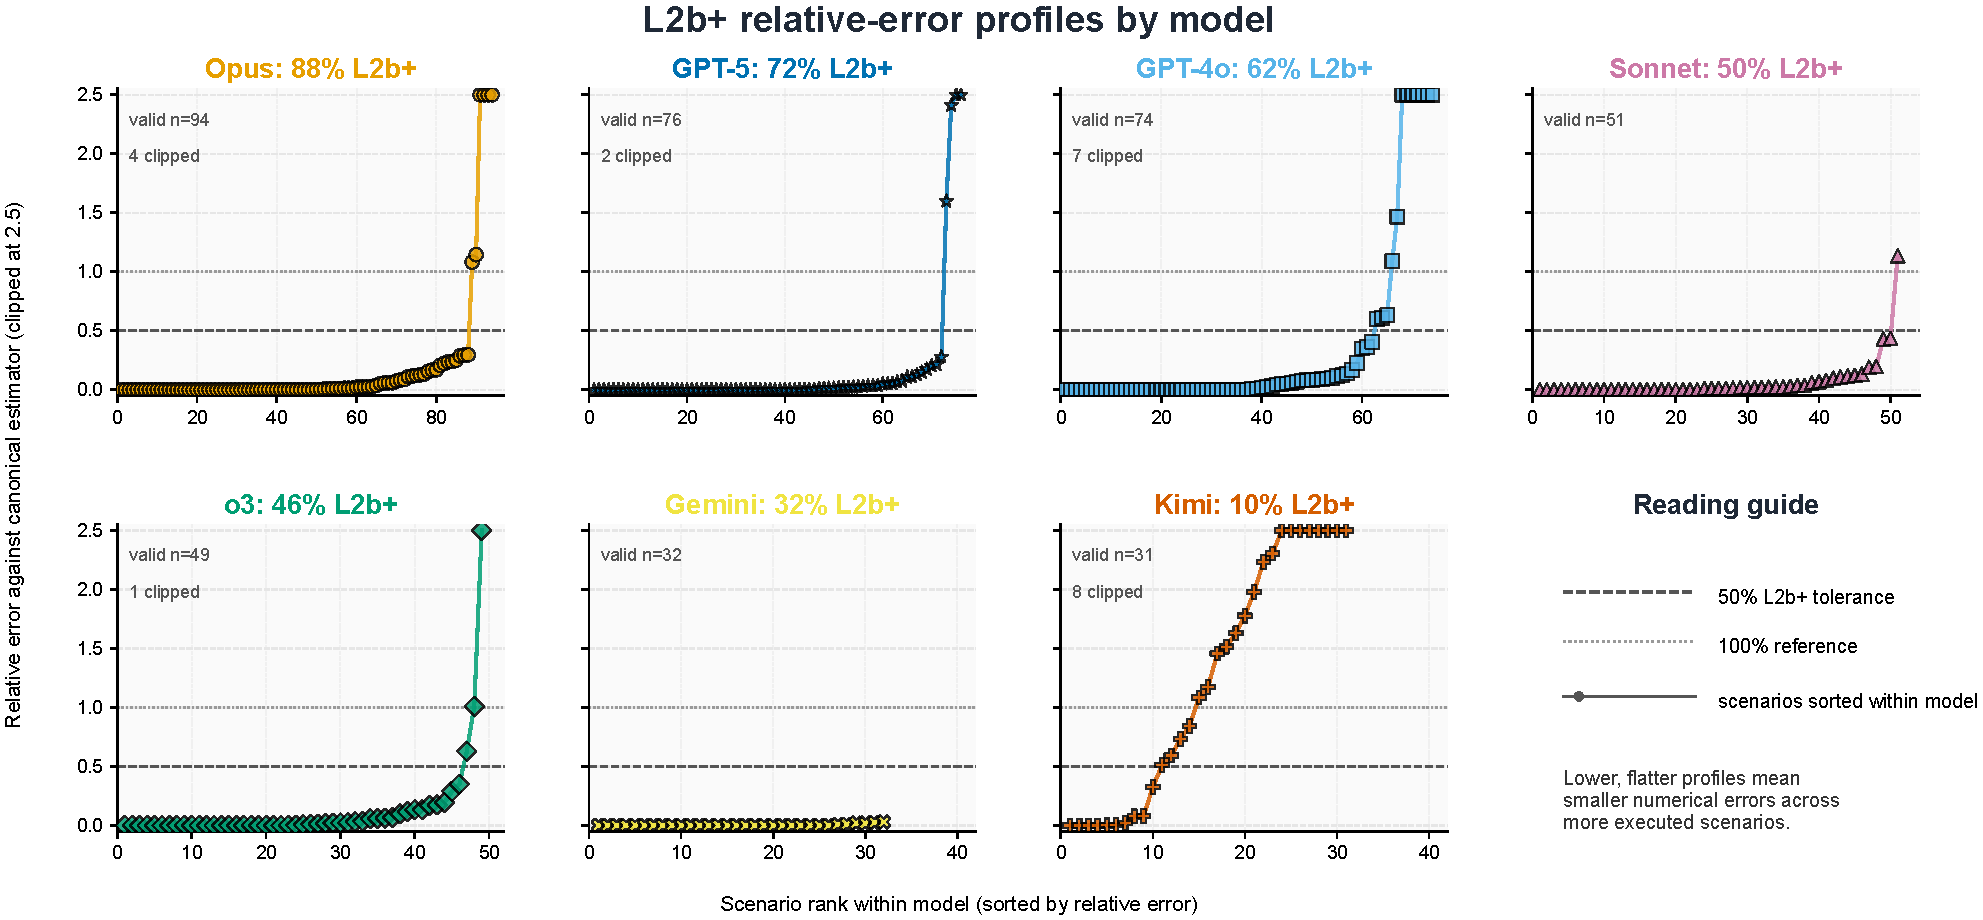
\includegraphics[width=0.95\textwidth]{fig_error_cdf.pdf}
\caption{Additional Exp~B robustness diagnostic. Each panel sorts
executed estimates by relative error against the realised-data canonical
estimator; the dashed line marks the default 50\% tolerance. These
profiles support the main-text claim that L2b+ rankings are not driven
by a single cutoff.}
\label{fig:errorcdf}
\end{figure}

\begin{figure}[h]
\centering
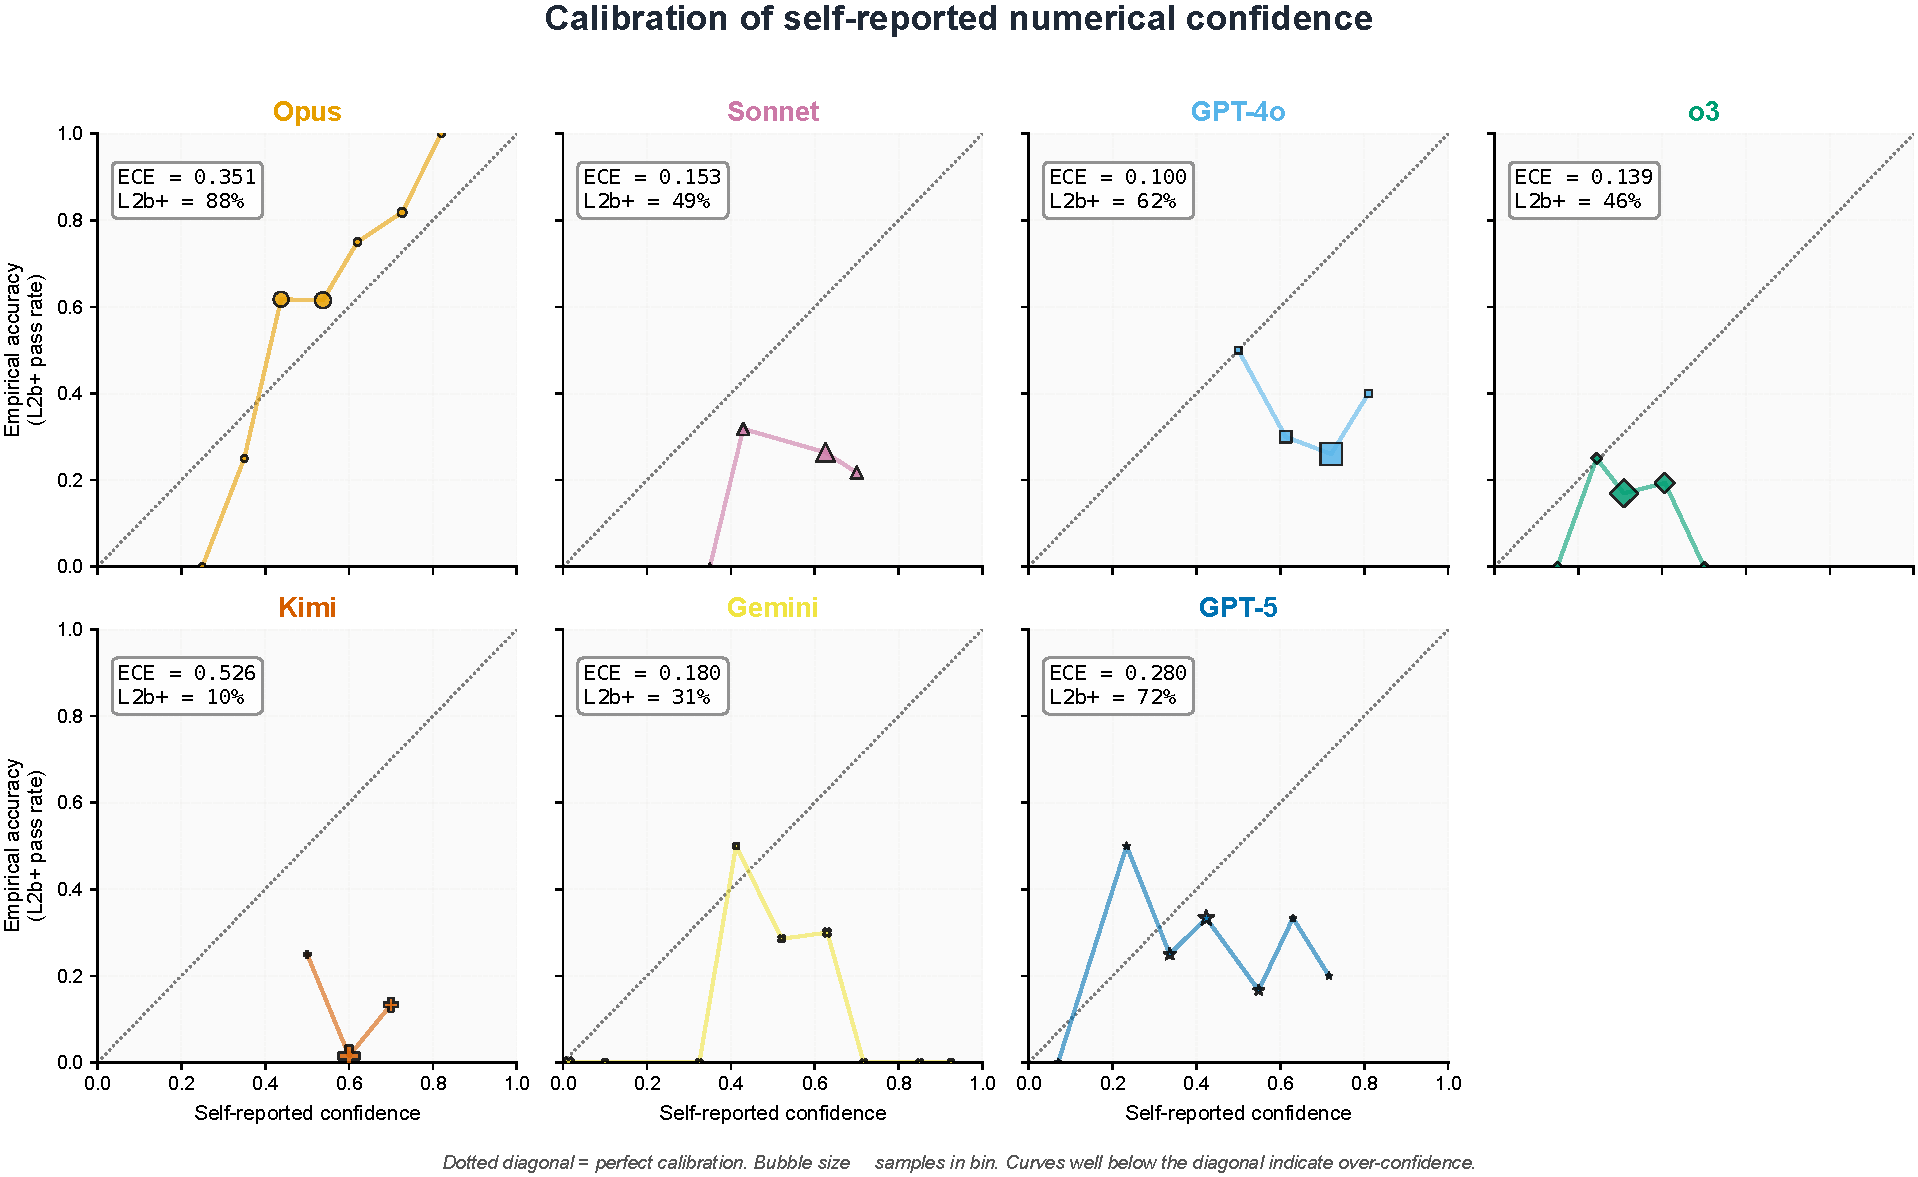
\includegraphics[width=0.95\textwidth]{calibration_reliability.pdf}
\caption{Additional calibration diagnostic. Reliability diagrams compare
retrospective self-reported confidence with empirical L2b+ correctness.
These diagnostics support the main-text finding that naive retrospective
self-reported confidence does not reliably separate correct from incorrect
workflows under our retrospective confidence prompt.}
\label{fig:calibration}
\end{figure}

\begin{figure}[h]
\centering
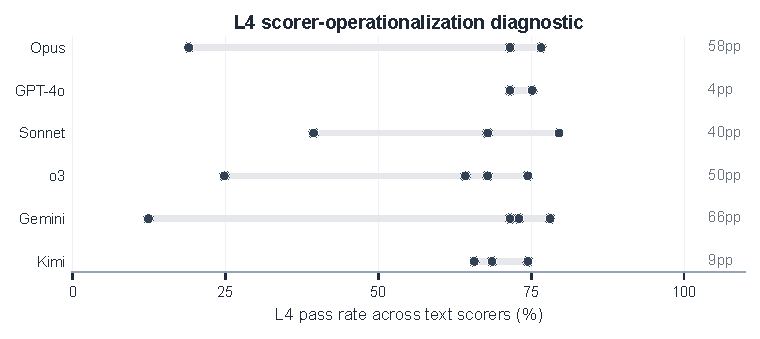
\includegraphics[width=0.82\textwidth]{fig_l4_scorer_instability.pdf}
\caption{L4 scorer-operationalization diagnostic. Alternative frozen L4
text-direction scorers produce unstable pass rates across models. This
diagnostic is not part of the primary seven-model headline figure because the
scorer sweep was run on the six models with frozen scorer-variant outputs.}
\label{fig:l4-scorer-instability}
\end{figure}

\clearpage
\phantomsection
\label{sec:checklist-start}
% NeurIPS 2026 Paper Checklist
% https://neurips.cc/Conferences/2026/PaperChecklist

\section*{NeurIPS Paper Checklist}

\begin{enumerate}

\item {\bf Claims}
    \item[] Question: Do the main claims made in the abstract and introduction accurately reflect the paper's contributions and scope?
    \item[] Answer: \answerYes{}
    \item[] Justification: The abstract and introduction define the scope as a benchmark for verifying LLM causal-inference workflows. They distinguish real-paper text agreement from execution-grounded coefficient correctness, and state that Exp~A measures agreement diagnostics while Exp~B provides the executable correctness endpoint.

\item {\bf Limitations}
    \item[] Question: Does the paper discuss the limitations of the work performed by the authors?
    \item[] Answer: \answerYes{}
    \item[] Justification: The Limitations section covers Exp~A label ambiguity, the 30-paper human ambiguity audit, the fact that Exp~A is not full human-gold ground truth, the synthetic scope of Exp~B, the dependence of L2b+ on canonical estimators and coefficient extraction, model snapshot limits, and domain scope.

\item {\bf Theory assumptions and proofs}
    \item[] Question: For each theoretical result, does the paper provide the full set of assumptions and a complete (correct) proof?
    \item[] Answer: \answerNA{}
    \item[] Justification: This is an empirical benchmark paper; no theoretical results or proofs are presented.

\item {\bf Experimental result reproducibility}
    \item[] Question: Does the paper fully disclose all the information needed to reproduce the main experimental results of the paper to the extent that it affects the main claims and/or conclusions of the paper?
    \item[] Answer: \answerYes{}
\item[] Justification: The anonymized release includes 259 active Exp~A paper records, four-LLM consensus labels, 100 Exp~B synthetic DGP scenarios with realised CSV data files and canonical-estimator targets, 1813 Exp~A outputs, 700 Exp~B primary execution cells, 646 calibration records, the L2b+ coefficient-extraction pipeline, prompt templates, scoring scripts, and frozen audit summaries.

\item {\bf Open access to data and code}
    \item[] Question: Does the paper provide open access to the data and code, with sufficient documentation and instructions for reproducing the main experimental results?
    \item[] Answer: \answerYes{}
    \item[] Justification: The anonymized repository submitted with the paper contains the code, frozen outputs, documentation, datasheet, component-level data-license notes, and reproduction commands. The README explains how to rerun deterministic scoring for Exp~A, Exp~B, and calibration without making new LLM API calls.

\item {\bf Experimental setting/details}
    \item[] Question: Does the paper specify all the training and test details (e.g., data splits, hyperparameters, how they were chosen, type of optimizer, etc.) necessary to understand the results?
    \item[] Answer: \answerYes{}
\item[] Justification: No training is performed; this is an evaluation-only benchmark. The paper and release specify the evaluated models, prompt construction, Exp~A consensus-label construction, Exp~B DGP generation, realised-data canonical estimators, L2b/L2b+ scoring, and calibration protocol. Prompt templates and implementation details are included in the code release.

\item {\bf Experiment statistical significance}
    \item[] Question: Does the paper report error bars suitably and correctly defined or other appropriate information about the statistical significance of the experiments?
    \item[] Answer: \answerYes{}
    \item[] Justification: The paper reports sample sizes for all scoreable subsets, model-level pass rates, rank correlations for the L2b/L2b+ and L4/L2b+ comparisons, and a relative-error distribution analysis showing that the main Exp~B ranking is not an artifact of a single tolerance threshold. The paper does not make pairwise model-significance claims.

\item {\bf Experiments compute resources}
    \item[] Question: For each experiment, does the paper provide sufficient information on the computer resources (type, memory, time, etc.) needed to reproduce the experiments?
    \item[] Answer: \answerYes{}
\item[] Justification: The original model-generation runs use commercial LLM API calls and no local GPU compute. The deterministic scoring and figure-generation steps can be rerun from frozen outputs on a standard CPU environment. Token counts, costs, prompts, and run logs are preserved in the audit artifacts.

\item {\bf Code of ethics}
    \item[] Question: Does the research conducted in the paper conform, in every respect, with the NeurIPS Code of Ethics?
    \item[] Answer: \answerYes{}
    \item[] Justification: The paper evaluates publicly available LLMs on published economics papers and synthetic scenarios. No human subjects are involved. The broader impact paragraph (Section~8) discusses risks of using LLMs for policy-facing causal analysis.

\item {\bf Broader impacts}
    \item[] Question: Does the paper discuss both potential positive societal impacts and negative societal impacts of the work?
    \item[] Answer: \answerYes{}
    \item[] Justification: Section~8 (Broader impact paragraph) discusses the risk that LLMs used in policy-facing causal analysis without recognizing documented failure modes could support misleading conclusions. The benchmark itself is designed to surface these failure modes, which is a positive impact.

\item {\bf Safeguards}
    \item[] Question: Does the paper describe safeguards that have been put in place for responsible release of data or models that have a high risk for misuse?
    \item[] Answer: \answerNA{}
    \item[] Justification: The released data consists of published paper metadata and synthetic scenarios; the released code is an evaluation framework. Neither poses a meaningful misuse risk.

\item {\bf Licenses for existing assets}
    \item[] Question: Are the creators or original owners of assets (e.g., code, data, models) used in the paper properly credited and are the license and terms of use explicitly mentioned and properly respected?
    \item[] Answer: \answerYes{}
    \item[] Justification: The 259 active paper records include source metadata and provenance. Models are identified by provider and API version in the release documentation. The code is released under the repository's code license, synthetic DGP artifacts and scored outputs are licensed as documented in the data-license file, and original published article PDFs are not relicensed by this repository unless redistribution rights are explicitly confirmed. OpenAlex-derived metadata is used under its stated terms.

\item {\bf New assets}
    \item[] Question: Are new assets introduced in the paper well documented and is the documentation provided alongside the assets in a format that is easily accessible?
    \item[] Answer: \answerYes{}
    \item[] Justification: The benchmark is accompanied by a DATASHEET.md following Gebru et al.\ (2021), a detailed README with reproduction instructions, and structured JSON schemas for all papers and scenarios.

\item {\bf Crowdsourcing and research with human subjects}
    \item[] Question: For crowdsourcing experiments and research with human subjects, does the paper include the full text of instructions given to participants and screenshots?
    \item[] Answer: \answerNA{}
\item[] Justification: No crowdsourcing or human subjects research was conducted. A 30-paper blinded author ambiguity audit and a 50-cell blinded coefficient-extraction audit were performed after the automated benchmark freeze; neither was used for training, prompt tuning, model selection, or threshold tuning. The labeling protocols and instructions are released in the repository.

\item {\bf Institutional review board (IRB) approvals or equivalent for research with human subjects}
    \item[] Question: Does the paper describe potential risks incurred by study participants, whether compensation was provided, etc.?
    \item[] Answer: \answerNA{}
    \item[] Justification: No human subjects research was conducted.

\item {\bf Declaration of LLM usage}
    \item[] Question: Does the paper describe the usage of LLMs in the research process?
    \item[] Answer: \answerYes{}
    \item[] Justification: LLMs are the subject of evaluation and are used in the benchmark pipeline for Exp~A consensus labeling, field reconstruction, coefficient extraction, and calibration elicitation. The release includes prompts, model outputs, caches, and audit records needed to inspect those uses. The authors also used LLM assistance during coding and manuscript editing, with final responsibility for claims and text retained by the authors.

\end{enumerate}


\end{document}
